\documentclass[letterpaper]{article} % DO NOT CHANGE THIS
\usepackage[submission]{aaai2027}  % DO NOT CHANGE THIS
\usepackage[hyphens]{url}  % DO NOT CHANGE THIS
\usepackage{graphicx} % DO NOT CHANGE THIS
\urlstyle{rm} % DO NOT CHANGE THIS
\def\UrlFont{\rm}  % DO NOT CHANGE THIS
\usepackage{natbib}  % DO NOT CHANGE THIS AND DO NOT ADD ANY OPTIONS TO IT
\usepackage{caption} % DO NOT CHANGE THIS AND DO NOT ADD ANY OPTIONS TO IT
\frenchspacing  % DO NOT CHANGE THIS
\usepackage{algorithm}
\usepackage{algorithmic}
\usepackage{booktabs}
\usepackage{amsmath}
\usepackage{amsthm}
\pdfinfo{
/TemplateVersion (2027.1)
}

\newtheorem{proposition}{Proposition}

\newcommand{\mcold}{\textsc{Cold}}
\newcommand{\mhint}{\textsc{Hint}}
\newcommand{\mfloor}{\textsc{Floor}}
\newcommand{\mfh}{\textsc{Floor+Hint}}
\newcommand{\mrep}{\textsc{Repair}}
\newcommand{\mlns}{\textsc{LNS}}
\newcommand{\mfo}{\textsc{F\&O-50}}
\newcommand{\mlb}{\textsc{LB-30}}
\newcommand{\mspt}{\textsc{SPT}}
\newcommand{\mmwkr}{\textsc{MWKR}}

\setcounter{secnumdepth}{0}

\title{Floor, Not Hint: Robust Solution Reuse for Anytime Rescheduling}
\author{
    Anonymous Submission
}
\affiliations{
}

\begin{document}

\maketitle

\begin{abstract}
When a scheduling problem changes---a job arrives, a machine fails---the schedule is typically recomputed by a solver under a tight time budget, and the previous schedule is commonly reused by passing it to the solver as a warm-start hint. We find this form of reuse unreliable: in the eight job-shop experimental campaigns in which we tested it, hinting CP-SAT with the previous solution significantly worsened anytime solution quality in two and significantly improved it in five. We study a simple alternative that keeps reuse outside the solver. A constructive repair of the previous schedule, which for job shops costs well under a millisecond, is kept as an anytime floor beside an unmodified solver run, and the better of the two is reported. By construction this never worsens the anytime curve of its own solver run. Empirically it reduced the primal integral significantly in all nine campaigns, on streams built from 84 published benchmark instances (five job-shop families and PSPLIB), against six reoptimization baselines including fix-and-optimize, large neighbourhood search and local branching, and with Gurobi and CPLEX in place of CP-SAT. Its gains concentrate on changes that perturb existing work and are smallest for job arrivals.
\end{abstract}

\section{Introduction}

Schedules in manufacturing and project management are rarely computed once. Jobs arrive or are cancelled, durations turn out longer than planned, and machines break down, so a schedule must be revised repeatedly, each time under a time limit set by the operational context \citep{vieira2003,ouelhadj2009}. Planning research has long asked whether such revisions should repair the previous plan or regenerate one from scratch \citep{nebel1995,vanderkrogt2005,fox2006}. When a modern constraint solver performs the revision, the question becomes concrete: how should the previous schedule be handed to the solver for the new instance?

The most common answer is a \emph{hint} (warm start): the previous solution is supplied to the solver as a suggested assignment for the variables that still exist. This changes the solver's own search, and we find that the effect of the change is unstable. In eight experimental campaigns on dynamic job-shop scheduling with CP-SAT \citep{cpsat}, hinting with the previous solution significantly \emph{worsened} anytime quality in two and significantly improved it in five; passing a repaired version of it as a hint, while also keeping the repair as a fallback, was significantly worse than no reuse at all in a further campaign.

We study an alternative that leaves the solver untouched. Before solving, a cheap constructive procedure repairs the previous schedule into a feasible schedule for the new instance; for job shops this takes under 0.4\,ms in our measurements. This repaired schedule is kept as an anytime \emph{floor} beside an unmodified, unhinted solver run on the new instance, and at every moment the better of the two is reported. We call the method \mfloor. Because the reported incumbent is a running minimum over the floor and the solver's own trajectory, \mfloor{} can never report a worse value than its own solver run would have at the same point of that run---an elementary property, which we state precisely because it is easy to overstate (it does \emph{not} imply that \mfloor{} never loses to an independently executed solver run).

Our contributions are empirical. Measuring anytime quality by the primal integral \citep{berthold2013}, we find that:
\begin{itemize}
\item \mfloor{} significantly improves on solving from scratch in all nine job-shop campaigns (it wins on 78.8--100\% of paired instances), whereas hint-based reuse changes sign across campaigns;
\item in the main campaign it has the lowest mean primal integral of ten methods and beats each of them head-to-head ($p < 10^{-30}$)---solver hints, fix-and-optimize, large neighbourhood search (LNS) seeded with the repaired schedule, approximate local branching, repair without a solver and two dispatching rules---except the variant that adds a hint to the floor, which it does not beat significantly;
\item the effect holds on streams built from published instances of five job-shop benchmark families and from PSPLIB project-scheduling instances, and when CP-SAT is replaced by Gurobi or CPLEX;
\item a breakdown by delta type shows where the difference comes from: after job arrivals, the repaired schedule fits the new instance poorly; used as a hint it significantly hurts, used as a floor it does not.
\end{itemize}

\section{Related Work}

\paragraph{Rescheduling.} Rescheduling has been surveyed for manufacturing systems \citep{vieira2003,ouelhadj2009} and, under uncertainty, for projects \citep{herroelen2005}. In match-up scheduling, part of the schedule is reconstructed after a disruption so that it matches up with the original schedule at some future time \citep{bean1991}. These methods change \emph{what} is re-optimized; \mfloor{} instead re-optimizes the full instance and uses the repaired schedule only as a fallback answer.

\paragraph{Plan reuse, repair and stability.} \citet{nebel1995} compared plan reuse with plan generation theoretically and empirically. \citet{vanderkrogt2005} extend planners to repair plans and report repair to be much more efficient than replanning from scratch. \citet{fox2006} argue that plan stability, a small difference between the old and the new plan, is a valuable property, and compare replanning with adapting the existing plan. Our floor is a repair in this sense, but we do not constrain the solver towards it; we report stability alongside quality.

\paragraph{Reoptimization in solvers.} The MIP Workshop 2023 computational competition addressed reoptimization, or warm starting, of mixed-integer programs after slight changes to their data, using information from previously solved instances \citep{bolusani2024}. Neighbourhood-based methods fix part of an incumbent and re-solve the rest, as in LNS \citep{shaw1998} and local branching \citep{fischetti2003}; BALANS selects LNS operators online with a multi-armed bandit \citep{cai2025}. We include fix-and-optimize, LNS and local-branching baselines that start from the repaired schedule or the previous solution.

\paragraph{Anytime evaluation.} Anytime algorithms can be interrupted at any point and return a result whose quality depends on the computation time \citep{dean1988,zilberstein1996}. We measure anytime quality with the primal integral \citep{berthold2013}, defined below.

\section{Problem Setting}

A \emph{stream} is a sequence of instances $I_0, I_1, \dots, I_T$ in which $I_t$ is obtained from $I_{t-1}$ by a \emph{delta}, e.g.\ a job arrival, a cancellation, a duration change or a machine outage. Each instance must be solved within a wall-clock budget $B$. A reuse method receives $I_t$ together with the solution $S_{t-1}$ that the \emph{same method} returned for $I_{t-1}$. Objectives are makespans to be minimized, except for knapsack, where the value is maximized.

During a solve, a method produces an anytime trajectory: $z(\tau)$ is the objective of its best solution found by time $\tau$, or undefined before its first solution. For instance $I_t$, let $z^*$ be the best objective found by any compared method. We use the gap $g(\tau) = (z(\tau) - z^*)/z^*$ (for knapsack, $(z^* - z(\tau))/z^*$), with $g(\tau) = 1$ before the first solution, and the normalized primal integral
\begin{equation}
\mathrm{PI} = \frac{1}{B}\int_0^B g(\tau)\,d\tau .
\end{equation}
Lower is better. The gap is not capped at 1, so a method whose solutions are more than twice as long as $z^*$ can have $\mathrm{PI} > 1$.

\section{Method}

\paragraph{Repair floor.} A domain-specific procedure $\rho(I_t, S_{t-1})$ turns the previous solution into a feasible solution for $I_t$ without calling a solver. For job shops, operations that survive the delta are sorted by their start time in $S_{t-1}$; operations of newly arrived jobs are appended, ordered by their position within their job. One pass then schedules each operation at the earliest time at which its job predecessor has finished and its machine is free, delaying it past any machine outage it would overlap. The result is feasible by construction for every delta type. For the resource-constrained project scheduling problem (RCPSP), $\rho$ is a serial schedule-generation pass \citep{kolisch1996} over a precedence-feasible activity list ordered by the previous start times, with new activities appended. For 0-1 knapsack, $\rho$ keeps the previously selected items that still exist, removes items in increasing value/weight order until the capacity holds, and then adds items greedily by value/weight.

\paragraph{Floor beside the solver.} \mfloor{} (Algorithm~\ref{alg:floor}) records the floor's objective as soon as it is built, then runs the solver on $I_t$ for the remaining budget with the same model, parameters and random seed as solving from scratch, and without any hint. The reported incumbent at every time is the better of the floor and the solver's best so far. On $I_0$ there is no previous solution and \mfloor{} reduces to the plain solver.

\begin{algorithm}[tb]
\caption{\mfloor: repair floor beside an unmodified solver run}
\label{alg:floor}
\textbf{Input}: instance $I_t$, previous solution $S_{t-1}$, budget $B$\\
\textbf{Output}: solution and trajectory for $I_t$
\begin{algorithmic}[1]
\STATE $F \leftarrow \rho(I_t, S_{t-1})$ \COMMENT{no solver call}
\STATE $\theta \leftarrow$ elapsed time; record $(\theta, f(F))$
\STATE run the solver on $I_t$ for $B-\theta$ seconds, unhinted; record each improving solution
\STATE report, at every time, the best solution recorded so far
\STATE \textbf{return} the best of $F$ and the solver's final solution
\end{algorithmic}
\end{algorithm}

\begin{proposition}
Let $z_C(\cdot)$ be the trajectory of the solver run inside \mfloor{} (started at time $\theta$), and $z_F(\cdot)$ the trajectory reported by \mfloor. Then $z_F(\theta + s) \le z_C(s)$ for every $s \in [0, B-\theta]$ at which $z_C(s)$ is defined. In particular, the final value of \mfloor{} is no worse than the final value of its own solver run, and its gap curve lies pointwise below that run's gap curve shifted by $\theta$.
\end{proposition}
\begin{proof}
The reported value at time $\theta + s$ is the minimum of the floor value and every objective the solver has reported by time $s$ of its run, which is at most $z_C(s)$.
\end{proof}

The proposition is elementary, and its scope matters. It compares \mfloor{} with \emph{its own} solver run, which starts $\theta$ seconds later than a solver started at time zero. It does not compare \mfloor{} with an independently executed solver run: under a wall-clock limit, two runs with the same seed can follow different trajectories, so an independent run can end with a better solution. We measure how often this happens below.

\paragraph{Cost.} We timed $\rho$ on all 450 stream instances of the main campaign's generator (Experimental Setup), 50 repetitions each, on the same machine as the experiments. Median construction time was 0.05, 0.10 and 0.18\,ms for $10{\times}10$, $15{\times}15$ and $20{\times}20$ job shops, with a maximum of 0.32\,ms, i.e.\ below 0.01\% of an 8\,s budget. Every constructed floor passed an independent feasibility check.

\section{Experimental Setup}

\paragraph{Job-shop streams.} Synthetic base instances are full job shops: $m$ jobs on $m$ machines, every job visiting every machine once in random order, durations uniform in $[5, 50]$. Deltas are drawn with weights 0.4 (arrival of a random new job), 0.2 (cancellation of a job), 0.25 (duration jitter of one job's operations) and 0.15 (an outage window on one machine). All streams are generated from a seed and are reproducible.

\paragraph{Campaigns.} The \emph{main} campaign uses $m \in \{10, 15, 20\}$, 15 streams per size, 10 deltas per stream and $B = 8$\,s, giving 495 instances per method (45 initial instances and 450 stream instances). Three further synthetic campaigns differ in size, budget and delta mix: \emph{pilot} ($m \in \{10,15\}$, $B \in \{1, 5, 10\}$\,s), \emph{arrivals} ($m=15$, $B = 5$\,s, arrival-type deltas only, four floor insertion rules), and the single-worker part of a \emph{workers} campaign ($m=15$, $B \in \{2, 8\}$\,s). Five campaigns use a published job-shop instance as the base of each stream, with deltas from the same generator (arriving jobs have 3--5 operations with durations in $[5,30]$) and $B=8$\,s: the OR-Library instances ft06, ft10, ft20, la01--la05, abz5 and abz6 \citep{beasley1990}, Taillard's ta01--ta20 \citep{taillard1993}, dmu01--dmu05 \citep{demirkol1998}, swv01--swv05 \citep{storer1992} and yn1--yn4 \citep{yamada1992}.

\paragraph{Methods.} Unless stated otherwise the solver is CP-SAT v9.15 with one worker and a fixed seed. \mcold{} solves each instance from scratch. \mhint{} passes $S_{t-1}$ to CP-SAT as a solution hint. \mfloor{} is our method; \mfh{} additionally passes the floor as a hint. \mrep{} returns the floor without solving. \mlns{} starts from the floor and runs 1\,s destroy-and-repair rounds with CP-SAT, cycling through four neighbourhoods (random, delta-touched, critical-path and outage-window operations, 25\% of operations each), keeping the machine order of non-destroyed operations. \mfo{} fixes the earliest-starting 50\% of operations at their floor start times and solves the rest with the floor as hint. \mlb{} is an approximate local branching: CP-SAT with $S_{t-1}$ as hint and a constraint allowing at most 30\% of surviving operations to change their start time. \mspt{} and \mmwkr{} are non-delay dispatching rules. On $I_0$, methods that need a previous solution start from \mspt{} or reduce to \mcold. Every returned solution is re-checked by an independent validator.

\paragraph{Statistics.} Methods are compared on identical instances. For each pair we report the share of paired instances on which a method has the lower PI, the exact two-sided sign test, and, where stated, a 95\% bootstrap confidence interval of the mean PI difference (2{,}000 resamples). P-values are Holm-corrected within each table. Experiments ran on a 20-thread Intel Core i7-12700 with up to 16 concurrent single-worker processes; all methods of a stream ran sequentially in the same process.

\section{Results}

\paragraph{Main campaign.} Table~\ref{tab:main} compares all methods on the 495 instances of the main campaign. \mfloor{} has the lowest mean PI and beats \mcold{} on 78.8\% of instances; its mean PI reduction is 0.0100 (95\% CI $[0.0086, 0.0114]$), i.e.\ 27\% of \mcold's mean PI. \mhint{} is significantly \emph{worse} than \mcold. Adding the hint to the floor (\mfh) does not help: its mean PI is higher than that of \mfloor, and head-to-head the two are not significantly different (\mfloor{} better on 52.1\% of instances, $p=0.37$). The neighbourhood-based baselines, which restrict the search around the repaired or previous solution, are far behind under this budget, and \mfloor{} beats each of them on at least 86.7\% of instances. \mrep{} alone is the worst method: it repairs its own previous repair at every step, and its mean final gap grows from 0.23 on initial instances to 1.68 after ten deltas. \mfloor{} avoids this accumulation because the schedule it repairs is the solver's output.

\begin{table}[t]
\centering
\small
\setlength{\tabcolsep}{4pt}
\begin{tabular}{lrrrr}
\toprule
Method & PI & Gap & W/L vs \mcold & $p$ \\
\midrule
\mfloor{} (ours) & \textbf{.0270} & \textbf{.0096} & 390/105 & $<10^{-38}$ \\
\mfh & .0337 & .0109 & 288/207 & .0003 \\
\mcold & .0370 & .0107 & -- & -- \\
\mhint & .0474 & .0139 & 187/308 & $1.2\cdot10^{-7}$ \\
\mlns & .0662 & .0367 & 121/374 & $<10^{-29}$ \\
\mfo & .1215 & .1188 & 65/430 & $<10^{-65}$ \\
\mmwkr & .1502 & .1499 & 1/494 & $<10^{-145}$ \\
\mlb & .2238 & .1496 & 27/468 & $<10^{-103}$ \\
\mspt & .2423 & .2421 & 0/495 & $<10^{-147}$ \\
\mrep & 1.0142 & 1.0141 & 0/495 & $<10^{-147}$ \\
\bottomrule
\end{tabular}
\caption{Main campaign (495 instances, $B=8$\,s). Mean primal integral (PI), mean final gap, wins/losses on PI against \mcold{} (no ties occurred) and Holm-corrected sign-test $p$-values.}
\label{tab:main}
\end{table}

\paragraph{Floor versus hint across campaigns.} Table~\ref{tab:consistency} repeats the comparison against \mcold{} in all nine job-shop campaigns. \mfloor{} wins significantly in every campaign. The two hint-based methods do not: \mhint{} loses significantly in the pilot and main campaigns and wins significantly on all five published-instance campaigns; \mfh{} loses significantly in the arrivals campaign (27.1\%) and is indistinguishable from \mcold{} in the pilot. The data do not tell us which property of a campaign decides the sign of the hint's effect; they do show that the sign is not stable, whereas the floor's is.

\begin{table}[t]
\centering
\small
\setlength{\tabcolsep}{3.5pt}
\begin{tabular}{lrrrr}
\toprule
Campaign & $n$ & \mfloor & \mfh & \mhint \\
\midrule
Pilot & 108 & 85.2* & 50.9\phantom{*} & 36.1$^\dagger$ \\
Arrivals & 288 & 86.8* & 27.1$^\dagger$ & -- \\
Workers (1 worker) & 28 & 100.0* & 75.0* & 42.9\phantom{*} \\
Main & 495 & 78.8* & 58.2* & 37.8$^\dagger$ \\
OR-Library & 540 & 89.3* & 83.9* & 70.6* \\
Taillard & 560 & 88.2* & 84.5* & 86.2* \\
DMU & 140 & 86.4* & 87.9* & 81.4* \\
SWV & 140 & 89.3* & 83.6* & 72.9* \\
YN & 112 & 83.9* & 65.2* & 62.5* \\
\bottomrule
\end{tabular}
\caption{Share (\%) of paired instances on which each reuse method has lower PI than \mcold{}, single-worker runs. * significant improvement, $^\dagger$ significant deterioration (sign test, Holm-corrected over the 26 tests, $\alpha=0.05$).}
\label{tab:consistency}
\end{table}

\begin{figure*}[t]
\centering
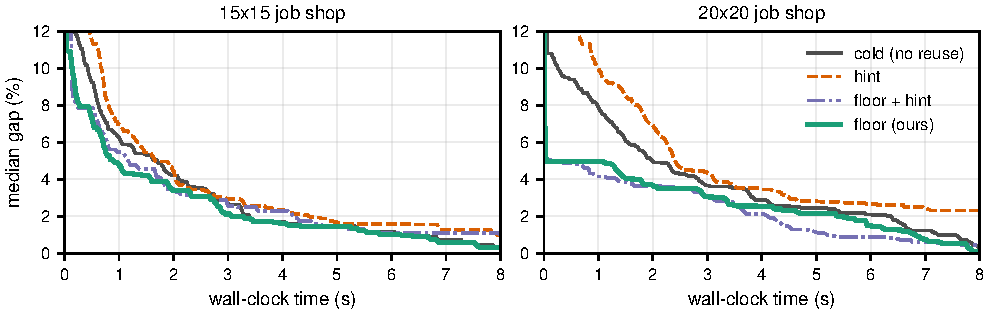
\includegraphics[width=0.95\textwidth]{figures/anytime}
\caption{Median gap to the best known value over time on the stream instances of six held-out streams per size (36 instances per size; seeds not used in any campaign; $B=8$\,s). The vertical axis is cut at 12\%; every curve is at 100\% before its first solution. The floor-based methods are ahead early in the run; the curves converge as the solver catches up.}
\label{fig:anytime}
\end{figure*}

\paragraph{Where reuse helps and where it hurts.} Figure~\ref{fig:anytime} shows the effect over time on held-out streams: at $\tau=1$\,s the median gap of \mfloor{} is 4.8\% ($15{\times}15$) and 5.0\% ($20{\times}20$), against 6.3\% and 7.9\% for \mcold{} and 7.0\% and 10.0\% for \mhint. In the main campaign the share of wins grows with size (65.5\%, 83.6\% and 87.3\% for $m = 10, 15, 20$). Table~\ref{tab:delta} breaks the main campaign down by delta type. After cancellations, duration jitter and outages, the repaired schedule is already close to the best known value (median gap 3.8--9.1\%) and \mfloor{} wins on 95--100\% of instances. After a job arrival, appending the new job gives a poor repaired schedule (median gap 52.2\%), and \mfloor{} gains little (59.5\%, not significant after correction). Hints behave differently. With the same poor repair as a hint, \mfh{} loses on 83.4\% of arrival instances, and \mhint, which passes the unrepaired previous solution, loses significantly after arrivals and after duration jitter. These results are consistent with a simple explanation: a floor that fits the new instance badly is soon overtaken by the solver and costs nothing, whereas a hint that fits badly biases the search. We have not tested this explanation directly. On initial instances, all three reuse methods run exactly the same solver call as \mcold; their non-significant win rates of 35.6--57.8\% show the run-to-run variability of a solver under a wall-clock limit.

\begin{table}[t]
\centering
\small
\setlength{\tabcolsep}{3.2pt}
\begin{tabular}{lrrrrr}
\toprule
Delta & $n$ & Floor gap & \mfloor & \mfh & \mhint \\
\midrule
Arrival & 163 & 52.2 & 59.5\phantom{*} & 16.6$^\dagger$ & 19.6$^\dagger$ \\
Cancellation & 106 & 5.0 & 95.3* & 86.8* & 79.2* \\
Duration jitter & 124 & 3.8 & 96.0* & 87.9* & 19.4$^\dagger$ \\
Outage & 57 & 9.1 & 100.0* & 77.2* & 36.8\phantom{*} \\
None (initial) & 45 & -- & 35.6\phantom{*} & 35.6\phantom{*} & 57.8\phantom{*} \\
\bottomrule
\end{tabular}
\caption{Main campaign by delta type. Floor gap: median gap (\%) of the repaired schedule itself to the best known value. Other columns: share (\%) of instances on which the method has lower PI than \mcold; * significant improvement, $^\dagger$ significant deterioration (sign test, Holm-corrected over the 15 tests).}
\label{tab:delta}
\end{table}

\paragraph{Final objective.} PI improvements do not come with worse final schedules on average (Table~\ref{tab:main}). Against an \emph{independent} \mcold{} run, \mfloor{}'s final makespan was better on 80, equal on 367 and worse on 48 of the 495 main-campaign instances; when worse, by a median of 0.73\% and at most 3.6\%. These losses are not excluded by the proposition, which concerns \mfloor's own solver run.

\paragraph{Stability.} In the spirit of plan stability \citep{fox2006}, we measured the share of operations present in both $S_{t-1}$ and $S_t$ whose start time changed. \mfloor{} changes 88.1\% of them versus 90.6\% for \mcold{}, so it is not materially more stable. Methods that constrain change are much more stable---27.8\% for \mlb, 44.1\% for \mfo, 70.0\% for \mlns---but, as Table~\ref{tab:main} shows, at a large cost in anytime quality under this budget.

\paragraph{Published benchmark instances.} Table~\ref{tab:real} reports the published-instance streams, including 40 PSPLIB RCPSP instances \citep{kolisch1997} (ten each from j30, j60, j90 and j120; three streams of six deltas per instance; deltas change durations or resource capacities, or insert or cancel activities; $B=8$\,s). Win rates lie between 83.9\% and 89.3\% for all six families. On the unchanged PSPLIB instances, all 40 have optimal makespans proven independently by two other solvers in a public benchmark comparison;\footnote{\url{https://optalcp.com/benchmarks/rcpsp/main.html}, comparing OptalCP and IBM CP Optimizer.} our runs reached the proven optimum in 222 of 240 cases, never reported a value below it, and missed it on only three instances (one each from j60, j90 and j120), by 2.1\% on average and at most 3.8\%. On a separate synthetic RCPSP campaign (60 activities, three resources with capacities 4--6, ten streams of eight deltas), \mfloor{} won on all 80 stream instances ($p < 10^{-23}$) and never ended with a worse makespan.

\begin{table}[t]
\centering
\small
\setlength{\tabcolsep}{4pt}
\begin{tabular}{llrrr}
\toprule
Family & Size & Inst. & $n$ & Win \% \\
\midrule
OR-Library & 36--100 ops & 10 & 540 & 89.3 \\
Taillard & 225, 300 ops & 20 & 560 & 88.2 \\
DMU & 300 ops & 5 & 140 & 86.4 \\
SWV & 200 ops & 5 & 140 & 89.3 \\
YN & 400 ops & 4 & 112 & 83.9 \\
PSPLIB & 30--120 act. & 40 & 840 & 87.1 \\
\bottomrule
\end{tabular}
\caption{Streams built from published instances: \mfloor{} versus \mcold. $n$ counts paired instances (all streams, all steps). All comparisons are significant ($p < 10^{-12}$, sign test).}
\label{tab:real}
\end{table}

\paragraph{Multiple workers.} CP-SAT is often run with several workers. In the small \emph{workers} campaign (28 paired instances per setting), \mfloor{} beat \mcold{} on 100\%, 82.1\%, 75.0\% and 82.1\% of instances with 1, 4, 8 and 16 workers (all $p \le 0.013$, uncorrected). \mhint{} won on 42.9\% with one worker but on 75.0--82.1\% with four or more, which is consistent with the instability of hints in Table~\ref{tab:consistency}. The sample is small and covers only $15{\times}15$ instances.

\paragraph{Other solvers.} The floor needs no access to solver internals, so we repeated the comparison with Gurobi 13.0 \citep{gurobi} and CPLEX 22.2 \citep{cplex}, using a disjunctive big-$M$ MIP model of the job shop \citep{manne1960,ku2016} and the standard 0-1 knapsack model. We could only use the free versions of these solvers, which reject models with more than 2{,}000 (Gurobi) or 1{,}000 (CPLEX) variables or constraints. The instances are therefore small: job shops with 6 machines, 10 initial jobs of 4--6 operations and four deltas ($B=8$\,s), and strongly correlated knapsacks with 700 items and four deltas ($B=5$\,s), six streams each. Table~\ref{tab:solvers} shows a significant improvement for every solver in both domains, and in all 180 comparisons the floor variant ended with the same final value as the same solver run from scratch. The three job-shop models returned identical final makespans on all 30 instances; on knapsack the solvers' final values differed by less than the default MIP optimality tolerance of $10^{-4}$. The solvers' own speed differs by domain: the job-shop MIP's mean PI was 7--9 times that of CP-SAT's interval model, whereas on knapsack CPLEX's was 40 times lower than CP-SAT's.

\begin{table}[t]
\centering
\small
\setlength{\tabcolsep}{3.5pt}
\begin{tabular}{llrrrr}
\toprule
Domain & Solver & PI \mcold & PI \mfloor & W/L & $p$ \\
\midrule
Job shop & CP-SAT & .00048 & .00022 & 24/6 & $1.4\cdot10^{-3}$ \\
 & Gurobi & .00422 & .00233 & 28/2 & $2.6\cdot10^{-6}$ \\
 & CPLEX & .00344 & .00165 & 25/5 & $6.5\cdot10^{-4}$ \\
Knapsack & CP-SAT & .01982 & .00435 & 29/1 & $2.9\cdot10^{-7}$ \\
 & Gurobi & .00299 & .00007 & 30/0 & $1.1\cdot10^{-8}$ \\
 & CPLEX & .00049 & .00015 & 29/1 & $2.9\cdot10^{-7}$ \\
\bottomrule
\end{tabular}
\caption{\mfloor{} with three solvers (30 paired instances per row; no ties). $p$: sign test, Holm-corrected over the six rows. Instance sizes are limited by the free solver licences.}
\label{tab:solvers}
\end{table}

\section{Limitations}

All budgets are wall-clock limits, and the campaigns ran several single-worker processes concurrently on one machine. This adds run-to-run variability, visible on initial instances where reuse methods reduce to \mcold, although all methods of a stream ran in the same process. The gap reference $z^*$ is the best value found by any compared method; apart from the unchanged PSPLIB instances, whose optima are known, we do not know how far it is from optimal. Every delta in our streams is synthetic: base instances are published benchmarks in six of our campaigns, but the changes applied to them are randomly generated rather than taken from real operations. The repair procedure is written per problem class. Job arrivals remain the weak case for job shops; in the arrivals campaign, three rules that insert new operations into idle machine gaps instead of appending them did not improve on appending (wins against \mcold{} on 84.7--87.5\% of instances versus 87.5\%; mean PI 0.0239--0.0247 versus 0.0238). The Gurobi and CPLEX experiments are small because of licence limits, and the knapsack experiments are close to trivial for these two solvers. Finally, the method improves the answer available at any given time; it does not make the solver prove optimality sooner, and against an independent solver run its final value is better or equal in most but not all cases.

\section{Conclusion}

A previous schedule can be reused by changing the solver's search or by keeping a repaired copy of it beside the search. In our experiments the first choice was unreliable---solver hints helped in some campaigns and hurt in others---while the second improved anytime quality in every campaign, on published benchmark instances, against neighbourhood-based reoptimization methods, and with three different solvers. Because it requires no change to the solver and, for job shops, a fraction of a millisecond, keeping the repair as a floor is a low-risk default for rescheduling under time limits, and a baseline that more elaborate reuse strategies should be compared against.

\bibliography{references}

\end{document}
